\documentclass{beamer}
\usepackage{tikz,amsmath,amssymb,amsfonts}
\newcommand{\ju}{{\scriptsize m USD }}
\renewcommand{\arraystretch}{1.5}
\newcommand{\fttheory}[1]{\fcolorbox{blue}{blue}{\color{white}\textbf{#1}\hspace{\textwidth}}}
\newcommand{\ftexampl}[1]{\fcolorbox{orange}{orange}{\color{black}\textbf{#1}\hspace{\textwidth}}}
\newcommand{\ftdata}[1]{\fcolorbox{violet}{violet}{\color{white}\textbf{#1}\hspace{\textwidth}}}
\newcommand{\ftheader}[1]{\fcolorbox{lightgray}{lightgray}{\color{black}\textbf{#1}\hspace{\textwidth}}}
\newcommand{\ftvocab}[1]{\fcolorbox{cyan}{cyan}{\color{black}\textbf{#1}\hspace{\textwidth}}}
\newcommand{\usd}{\text{ {\scriptsize USD}}}
\newcommand{\eur}{\text{ {\scriptsize EUR}}}
\newcommand{\aud}{\text{ {\scriptsize AUD}}}
\newcommand{\mxn}{\text{ {\scriptsize MXN}}}
\newcommand{\musd}{\text{ m {\scriptsize USD}}}
\newcommand{\meur}{\text{ m {\scriptsize EUR}}}
\newcommand{\maud}{\text{ m {\scriptsize AUD}}}

\begin{document}

\begin{frame}
\begin{center}
\Huge Lecture 0.1: \\
Introduction
\end{center}
\end{frame}

\begin{frame}{\ftheader{Lecture 0.1: Introduction}}
	\begin{itemize}
		\item Revisit and revamp NPV
		\item Distinguish speculation from investing
		\item Explore asset classes and the markets in which they trade
		\item Discuss basic market operations (shorting, leverage, arbitrage)
	\end{itemize}
\end{frame}

\begin{frame}
\begin{center}
\Huge NPV Revisited
\end{center}
\end{frame}

\begin{frame}{\fttheory{NPV Revisited}}
	\begin{itemize}
		\item \underline{Finance} is the study of investment/divestment decisions
		\item E.g. buy a stock, sell a house, build a factory
		\item We use the Net Present Value (NPV) to make such decisions 
		\item E.g. consider a security that pays $10\musd$ in one year (could be a stock paying dividends or a bond paying coupons). It costs $7.5\musd$ and the rate of return on another security of equivalent risk is $2\%$. You know that 
		\begin{equation}
			\boxed{
			\text{NPV}=-7.5\musd+\frac{10\musd}{1.02}\approx 2.3\musd
			}
		\end{equation}
		You should invest ($10\musd$ vs. $1.02\times7.5\musd$) 
		\item Stocks, bonds, and derivatives are not so simple
	\end{itemize}
\end{frame}

\begin{frame}{\fttheory{What if the NPV is negative?}}
	\begin{itemize}
		\item You can't sell a factory that you don't own, but you \textit{can} sell a stock/bond/derivative that you don't own
		\item Suppose that the security costs $12\musd$
		\item The NPV would seem to be negative
		\item Solution: borrow the security, sell it for $12\musd$, invest the proceeds at $2\%$. In one year, repay the lender $10\musd$.
		\item In this case, the NPV is 
		\begin{equation}
			\boxed{
			\text{NPV}=+12\musd-\frac{10\musd}{1.02}\approx2.2\musd
			}
		\end{equation}
		\item This is called \textit{shorting}
	\end{itemize}
\end{frame}

\begin{frame}{\fttheory{What if everyone wants the investment?}}
	\begin{itemize}
	\item Consider the original example:
		\begin{equation}
			\boxed{
			\text{NPV}=-7.5\musd+\frac{10\musd}{1.02}>0.
			}
		\end{equation}
	\item The $7.5\musd$ is the price of the investment
	\item If someone paid $8.5\musd$ instead of $7.5\musd$, their NPV would still be positive
	\item In fact, an investor could pay up to $\approx9.8\musd$ and their NPV would still be positive 
	\item This observation will enable us to compute the prices of all sorts of financial securities, including derivatives
	\item This is called \textit{no-arbitrage pricing}
	\end{itemize}
\end{frame}

\begin{frame}{\fttheory{What if different terms have different yields?}}
	\begin{itemize}
	\item Suppose instead that the security pays $10\musd$ in one year and $10\musd$ in two years
	\item What rate do we use?
	\item If the return on one-year debt is 1\% and the return on two-year debt is 3\%, then 
		\begin{equation}
			\boxed{
			\text{NPV}=-7.5\musd+\frac{10\musd}{1.01}+\frac{10\musd}{1.03^2}
			}
		\end{equation}
	\item This is called \textit{the term-structure} (or \textit{yield curve})
	\end{itemize}
\end{frame}

\begin{frame}{\fttheory{Other questions}}
	\begin{itemize}
		\item What if you finance your investment with debt?
		\item What if cash-flows are risky?
		\item What about the state of the economy?
	\end{itemize}
\end{frame}


\begin{frame}
\begin{center}
\Huge Speculation vs. Investing
\end{center}
\end{frame}


\begin{frame}{\fttheory{Two Hats}}
	\begin{itemize}
		\item Think about wearing one of two hats:  \underline{investor} or \underline{speculator}
		\item Investors want to passively earn a return on their investments
		\item They trade so that they can share risk with other investors
		\item Speculators want to exploit small mispricings (hard to find)
		\item They trade so that they can buy from (sell to) other speculators or investors with worse information
	\end{itemize}
\end{frame}

\begin{frame}{\fttheory{Speculator Hat: \textit{where do trading profits come from?}}}
	\begin{itemize}
		\item Trading (as typically understood) is a zero-sum game
		\item Ann \underline{knows} that stock $X$ is worth \$20
		\item Bob \underline{thinks} that $X$ is worth \$15
		\item Ann buys $X$ from Bob at \$15 and makes \$5
		\item At the end of the day, Mary at the factory was the only one who actually did any work
		\item Conclusion: people can make money trading
		\item However, acquiring information requires a lot of time and money, and even the best fail (e.g. LTCM, Great Recession)
	\end{itemize}
\end{frame}

\begin{frame}{\fttheory{Investor Hat}}
	\begin{center}
		\renewcommand{\arraystretch}{1.5}
		\begin{tabular}{cc|cc}
			\multicolumn{2}{c}{\textbf{Bet A}} & \multicolumn{2}{c}{\textbf{Bet B}} \\
			Amount & Probability & Amount & Probability \\ \hline
			-\$10,000 & 0.001 & -\$10 & 1. \\
			\$0 & 0.999 & & \\ \hline
			\multicolumn{2}{c}{Average = -\$10} & \multicolumn{2}{c}{Average = -\$10}
		\end{tabular}
	\end{center}
\begin{center}
Which do you prefer?
\end{center}
\pause
\begin{itemize}
	\item If you preferred \textbf{Bet B} to bet \textbf{Bet A} you are \underline{risk-averse}, \textbf{Bet A} to bet \textbf{Bet B}, you are \underline{risk-loving}, while if you were indifferent, you are \underline{risk-neutral}
	\item Our theory of investments rests on the observation that investors are risk-averse
\end{itemize}
\end{frame}

\begin{frame}{\fttheory{Investor Hat}}
	\begin{itemize}
		\item Trading allows people to \underline{share risk}
		\item 100\% of Ann’s portfolio is in Exxon Mobil (XOM)
		\item 100\% of Bob’s portfolio is in Apple (AAPL)
		\item Let Ann and Bob trade so that they each have portfolios with 50\% in XOM and 50\% in AAPL
		\item It turns out that Ann and Bob reduce risk without sacrificing return. We’ll work out the math on this one later.
	\end{itemize}
\end{frame}

\begin{frame}
\begin{center}
\Huge ``Asset'' Classes
\end{center}
\end{frame}

\begin{frame}{\ftvocab{Basic Vocabulary}}
	\begin{itemize}
		\item An \underline{asset} is anything that produces something in the future
		\item Examples: tractor, milk cow
		\item A \underline{security} is a claim to the output of an asset
		\item Examples: stock, bond
		\item I will often refer to the study of investments as asset pricing
	\end{itemize}
\end{frame}

%-------------------------------------------------------------------------%
% overview
%-------------------------------------------------------------------------%
\begin{frame}{\fttheory{Cash-Bonds-Stocks: An Asset-Based Perspective}}
	\begin{itemize}
		\item Remember that \underline{assets} produce something of value, while \underline{securities} are claims to the output of the asset
		\item The value of a firm's assets is uncertain, and depends on how well the firm performs, the state of the economy, and so on
		\item Suppose an investor's portfolio contains some cash, some of the firm's bonds, and some of its stock
		\item How does the value of her portfolio vary with the value of the firm's assets?
	\end{itemize}
\end{frame}

\begin{frame}{\fttheory{Cash-Bonds-Stocks: An Asset-Based Perspective}}
	\begin{center}
		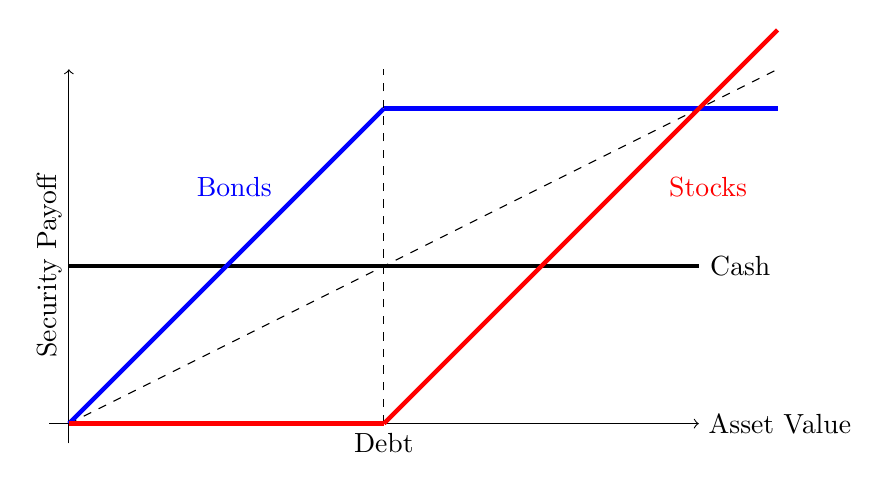
\begin{tikzpicture}
			\draw[->] (-.25,0) -- (8,0) node[anchor=west]{Asset Value};
			\draw[->] (0,-.25) -- (0,4.5);
			\draw[dashed] (4,0) node[anchor=north]{Debt} -- (4,4.5);
			\draw[dashed] (0,0) -- (9,4.5);
			\draw (-.25,2) node[rotate=90]{Security Payoff};
			% cash
			\draw[ultra thick] (0,2) -- (8,2) node[anchor=west]{Cash};
			% bonds
			\draw[ultra thick,color=blue] (0,0) -- (4,4);
			\draw[ultra thick,color=blue] (4,4) -- (9,4);
			\draw (1.5,3) node[anchor=west]{\color{blue}Bonds};
			% stocks
			\draw[ultra thick,color=red] (0,0) -- (4,0);
			\draw[ultra thick,color=red] (4,0) -- (9,5);
			\draw (7.5,3) node[anchor=west]{\color{red}Stocks};
		\end{tikzpicture}
	\end{center}
\end{frame}

\begin{frame}{\fttheory{Cash-Bonds-Stocks: An Asset-Based Perspective}}
	\begin{center}
		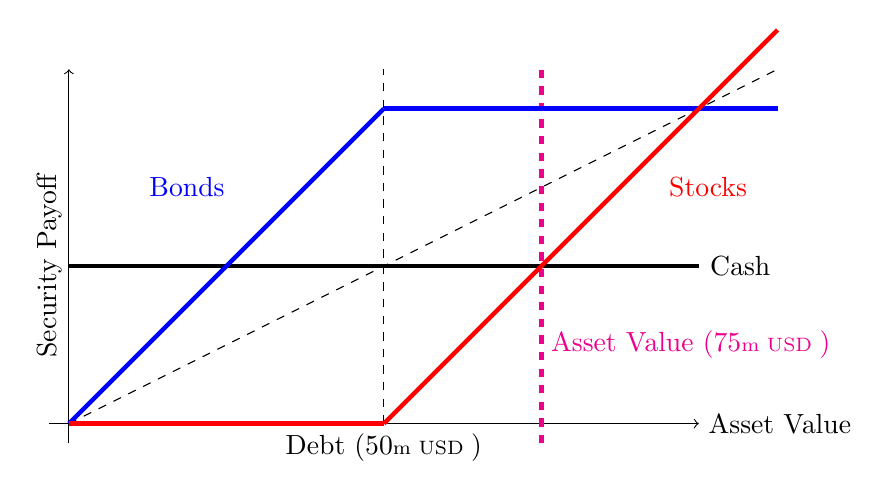
\begin{tikzpicture}
			\draw[->] (-.25,0) -- (8,0) node[anchor=west]{Asset Value};
			\draw[->] (0,-.25) -- (0,4.5);
			\draw[dashed] (4,0) node[anchor=north]{Debt (50\ju)} -- (4,4.5);
			\draw[dashed] (0,0) -- (9,4.5);
			\draw (-.25,2) node[rotate=90]{Security Payoff};
			% asset value
			\draw[dashed,ultra thick,color=magenta] (6,-.25) -- (6,4.5);
			\draw (6,1) node[anchor=west]{\color{magenta}Asset Value (75\ju)};
			% cash
			\draw[ultra thick] (0,2) -- (8,2) node[anchor=west]{Cash};
			% bonds
			\draw[ultra thick,color=blue] (0,0) -- (4,4);
			\draw[ultra thick,color=blue] (4,4) -- (9,4);
			\draw (1.5,3) node{\color{blue}Bonds};
			% stocks
			\draw[ultra thick,color=red] (0,0) -- (4,0);
			\draw[ultra thick,color=red] (4,0) -- (9,5);
			\draw (7.5,3) node[anchor=west]{\color{red}Stocks};
		\end{tikzpicture}
	\end{center}
\end{frame}

\begin{frame}{\fttheory{Cash-Bonds-Stocks: An Asset-Based Perspective}}
	\begin{center}
		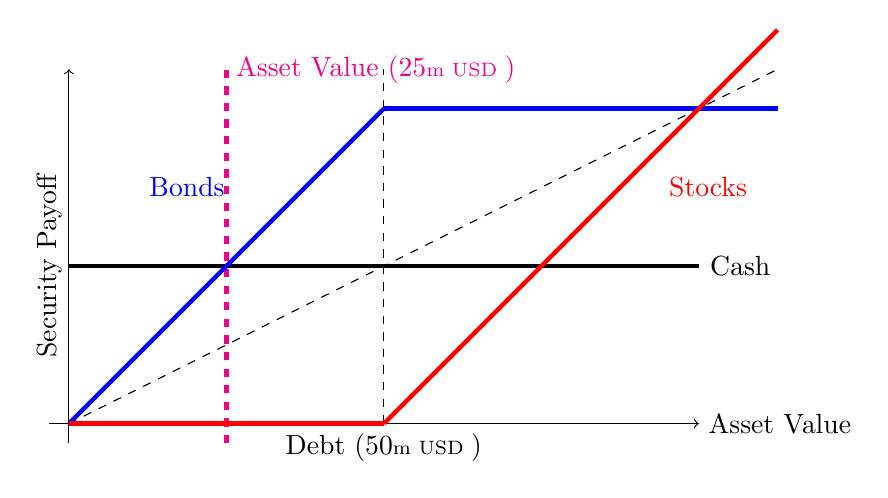
\begin{tikzpicture}
			\draw[->] (-.25,0) -- (8,0) node[anchor=west]{Asset Value};
			\draw[->] (0,-.25) -- (0,4.5);
			\draw[dashed] (4,0) node[anchor=north]{Debt (50\ju)} -- (4,4.5);
			\draw[dashed] (0,0) -- (9,4.5);
			\draw (-.25,2) node[rotate=90]{Security Payoff};
			% asset value
			\draw[dashed,ultra thick,color=magenta] (2,-.25) -- (2,4.5);
			\draw (2,4.5) node[anchor=west]{\color{magenta}Asset Value (25\ju)};
			% cash
			\draw[ultra thick] (0,2) -- (8,2) node[anchor=west]{Cash};
			% bonds
			\draw[ultra thick,color=blue] (0,0) -- (4,4);
			\draw[ultra thick,color=blue] (4,4) -- (9,4);
			\draw (1.5,3) node{\color{blue}Bonds};
			% stocks
			\draw[ultra thick,color=red] (0,0) -- (4,0);
			\draw[ultra thick,color=red] (4,0) -- (9,5);
			\draw (7.5,3) node[anchor=west]{\color{red}Stocks};
		\end{tikzpicture}
	\end{center}
\end{frame}

\begin{frame}
\begin{center}
\Huge Asset Markets
\end{center}
\end{frame}

%=============================================================================%
%   MARGIN, SHORTING, AND ARBITRAGE                                           %
%=============================================================================%
\begin{frame}{\fttheory{Asset Markets}}
	In this section, we cover different types of markets and basic market operations
	\begin{enumerate}
		\item\textbf{Types of Markets}: direct search, brokered, dealer, and auction markets
		\item\textbf{Leverage} involves borrowing money to finance the purchase of a security
		\item\textbf{Shorting} means borrowing a security, selling it, buying it again, and returning it to its owner
		\item\textbf{Arbitrage} means profiting from the mispricing of two or more securities
		\item\textbf{Orders}: market, limit buy/sell, stop-loss buy/sell
	\end{enumerate}
\end{frame}

%=============================================================================%
%   SECURITIES MARKETS                                                        %
%=============================================================================%
\begin{frame}{\fttheory{Types of Markets}}
	\begin{enumerate}
		\item \textbf{Direct Search Markets}
		\begin{itemize}
			\item Buyers and sellers locate one another on their own 
		\end{itemize}
			\item \textbf{Brokered Markets}
		\begin{itemize}
			\item Third party assists in locating buyer or seller (e.g. realtors in housing, investment banks in corporate transactions)
			\item Does not hold inventory
		\end{itemize}
		\item \textbf{Dealer Markets}
		\begin{itemize}
			\item Third party acts as intermediate buyer or seller (e.g. cars, corporate bonds)
			\item Holds inventory
		\end{itemize}
		\item \textbf{Auction Markets}
		\begin{itemize}
			\item Brokers and dealers trade in one location (e.g. stocks, currencies, Treasuries)
			\item Trading is more or less continuous
		\end{itemize}
	\end{enumerate}
\end{frame}

%=============================================================================%
%   MARGIN                                                                    %
%=============================================================================%
\begin{frame}{\fttheory{Leverage}}
\begin{itemize}
\item Investors can borrow from financial institutions to finance the purchase of securities
\item Investors who do so are said to be using \underline{leverage} 
\item Historically, buying stocks with leverage has been referred to as \textit{buying on margin} where \underline{margin} refers to the equity the investor contributes to the purchase
\end{itemize}
\end{frame}

%=============================================================================%
%   MARGIN                                                                    %
%=============================================================================%
\begin{frame}{\ftdata{Leverage: Practical Considerations}}
\begin{itemize}
\item Retail investors face \underline{margin requirements} that restrict the amount that they can borrow
\item Institutional investors (e.g. pension, mutual, hedge funds) negotiate terms with the institutions from which they borrow
\item There are two margin requirements
\vfill
\item [1.] Initial Margin Requirement (IMR)
\begin{itemize}
\item Minimum percent of initial investor equity
\item Set by Fed under Reg T, currently 50\% for stocks
\end{itemize}
\item [2.] Maintenance Margin Requirement (MMR)
\begin{itemize}
\item Minimum amount equity can be before additional funds must be put into account
\item Exchanges mandate minimum MMR of 25\%
\end{itemize}
\vfill
\item A broker makes a \underline{margin call} when she informs the investor that he must either put up more equity or liquidate his position
\end{itemize}
\end{frame}

\begin{frame}{\ftexampl{Leverage}}
	\small
	Let's start with a toy example. Suppose you have 50 USD and you want to buy a 100 USD stock. You can borrow at 10\% for one year. What happens if the stock rises to 120 USD in one year? What if it falls to 80 USD? Describe the balance sheet.
		\pause
		\begin{itemize}
			\item{\color{blue} Initially, you have 100 USD in assets, 50 USD in liabilities, and 50 USD in equity (margin).}
			\item{\color{blue} If the stock rises to 120 USD ($+20\%$), then your have 120 USD in assets, 55 USD in liabilities, and 65 USD in equity (margin). Your return was $(65-50)/50=+30\%$ (compare with $+20\%$).}
			\item{\color{blue} If the stock falls to 80 USD ($-20\%$), then your have 80 USD in assets, 55 USD in liabilities, and 25 USD in equity (margin). Your return was $(25-50)/50=-50\%$ (compare with $-20\%$).}
			\item{\color{blue} Conclusion: leverage magnifies returns}
		\end{itemize}
\end{frame}

%============================================================================%
%   MARGIN                                                                   %
%============================================================================% 
\iffalse
\begin{frame}{\ftexampl{Leverage}}
	\small
	On 2008-01-31, Microsoft (MSFT) traded for 32.6 USD. Suppose you bought 1,000 shares with 20,000 USD of capital. What was your margin in percent and in USD? Did it satisfy the IMR? As of 2008-02-29, the value of your position fell 16.2273\% (accounting for dividends). What was your margin in percent and in USD? Did it satisfy the MMR? What was your return in percent? Assume you can borrow at 9.569\% APR\footnote{This (example) rate comes from TD. Remember to divide by 12.}.  
	\pause
		\begin{enumerate}
			\item{\color{blue}Your position (assets) was 32,600 USD. You borrowed 12,600 USD (liabilities). Your margin is 20,000 USD (equity) or 61.3497\% (equity over assets). Your margin satisfied the IMR.}
			\item{\color{blue}The new value of your position (assets) was 27,309.9002 USD and your new liability was 20,159.4833. Your margin is assets minus liabilities (equity): 7150.4169 USD or 26.1825\%. Your margin satisfied the MMR.}
		\end{enumerate}
\end{frame}
\fi
\begin{frame}{\ftexampl{Leverage}}
	\small
	On 2008-01-31, Microsoft (MSFT) traded for 32.6 USD. Suppose you bought 1,000 shares with 20,000 USD of capital. What was your margin in percent and in USD? Did it satisfy the IMR? As of 2008-02-29, the value of your position fell 16.2273\% (accounting for dividends). What was your margin in percent and in USD? Did it satisfy the MMR? Assume you can borrow at 9.569\%\footnote{This (example) rate comes from TD}.  
	\pause
		\begin{enumerate}
			\item{\color{blue}Your position (assets) was 32,600 USD. You borrowed 12,600 USD (liabilities). Your margin is 20,000 USD (equity) or 61.3497\% (equity over assets). Your margin satisfied the IMR.}
			\item{\color{blue}The new value of your position (assets) was 27,309.9002 USD and your new liability was 12,700.4745 USD. Your margin is assets minus liabilities (equity): 14,609.4257 USD or 53.495\%. Your margin satisfied the MMR.}
		\end{enumerate}
\end{frame}


%============================================================================%
%   SHORTING                                                                 %
%============================================================================% 
\begin{frame}{\fttheory{Shorting}}
\begin{itemize}
\item \underline{Shorting} involves borrowing a security, selling it, buying it again, and returning it to its owner
\item \textit{It should be as if the person who lent you the security never lent you the security. All dividends, coupon payments, etc. should paid to the lender during the life of the trade.}
\item \underline{Long position}: buy first, sell later; bullish: bet on price increase, buy low, sell high
\item \underline{Short position}: sell first, buy later; bearish: bet on price decrease, sell high, buy low
\end{itemize}
\end{frame}

%============================================================================%
%   SHORTING                                                                 %
%============================================================================% 
\section{Shorting}
\begin{frame}{\ftdata{Shorting: Practical Considerations}}
\begin{itemize}
\item If you borrow the security from an institution, you will most likely need to post margin 
\item The institution sells the security, deposits the proceeds, and deposits your margin into a margin account 
\item You cannot withdraw the proceeds until you ``cover'' 
\item When you \underline{cover} your position, you buy the security in the market and transfer it to the institution 
\item We will abstract from these issues in much of the course
\end{itemize}
\end{frame}

%============================================================================%
%   SHORTING                                                                 %
%============================================================================% 
\begin{frame}{\ftexampl{Shorting}}
	\small
	Let's continue with the Microsoft example. Recall that on 2008-01-31, Microsoft traded for 32.6 USD. On 2008-02-29, MSFT traded for 27.2 USD and had paid a dividend of 0.11 USD. What was your profit/loss per share? What if Microsoft had risen to 35 USD?

	\pause
	\begin{itemize}
		\item {\color{blue} You made a profit of $32.6\text{ USD}-27.2\text{ USD}-0.11\text{ USD}=5.29\text{ USD}$}
		\item {\color{blue} If the stock had risen to 35 USD, you would have suffered a loss of $32.6\text{ USD}-35\text{ USD}-0.11\text{ USD}=-2.51\text{ USD}$}
		\item {\color{blue}In both cases, the institution from which you borrowed the shares received the same cash flows it would have received had it not lent you the shares}
	\end{itemize}
\end{frame}

%=============================================================================%
%   CLEARINGHOUSE                                                             %
%=============================================================================%
\iffalse
\begin{frame}{Application: Clearinghouses}
	\begin{center}
		\textbf{TODO: include discussion (possible figure) about clearinghouse from Chapter 17 (pg. 551)}
	\end{center}
\end{frame}
\fi

%============================================================================%
%   ARBITRAGE                                                                %
%============================================================================% 
\begin{frame}{\fttheory{Arbitrage}}
\begin{itemize}
\item What if the same security trades for different prices in different markets?
\item Suppose gold trades for 850 in New York and 900 in London.
\item You \underline{buy} for 850 in New York, \underline{sell} for 900 in London, make 50. 
\item New York is flooded with buy orders and London is flooded with sell orders. Prices eventually equalize.
\end{itemize}
\end{frame}

%============================================================================%
%   ARBITRAGE                                                                %
%============================================================================%
\begin{frame}{\ftexampl{Arbitrage}}
\begin{itemize}
\item On 2020-01-28, the yield on a one year T-bill was 1.53\%. 
\item What's the fair price?
\begin{align*}
	\text{price}=\frac{100\text{ USD}}{1+.0153}=98.4931\text{ USD}
\end{align*}
\item Because T-bills are risk-free, we ignore margin requirements
\item Assume that you can borrow from and lend to a counterparty (call it a ``bank'') for a year at 1.53\%
\end{itemize}
\end{frame}

%============================================================================%
%   ARBITRAGE                                                                %
%============================================================================%
\begin{frame}{\ftexampl{Arbitrage}}
\begin{itemize}
\item What if the T-bill is trading for 97.5082 USD? 
\item Cash Flow Table
\begin{table}
\begin{center}
\begin{tabular}{lrr}
	& \textbf{2020-01-28} & \textbf{2021-01-28} \\ \hline
	Buy the T-bill & -97.5082 USD & +100 USD \\
	Bank & +98.4931 USD & -100 USD\\ \hline
	Net Cash Flow & +.9849 USD & 0 USD 
\end{tabular}
\end{center}
\end{table}
\item Borrow 98.4931 USD, use 97.5082 USD of it to buy the T-bill
\item In one year's time, you'll owe the bank 100 USD but the T-bill will pay you 100 USD
\end{itemize}
\end{frame}

%============================================================================%
%   ARBITRAGE                                                                %
%============================================================================%
\begin{frame}{\ftexampl{Arbitrage}}
\begin{itemize}
\item What if the T-bill is trading for 99.4780 USD?
\item Cash Flow Table
\begin{table}
\begin{center}
\begin{tabular}{lrr}
& \textbf{2020-01-28} & \textbf{2021-01-28} \\ \hline
Sell the Bond & +99.4780 USD & -100 USD \\
Deposit the Proceeds & -98.4931 USD & +100 USD \\ \hline
Net Cash Flow & +.9849 USD & 0 USD
\end{tabular}
\end{center}
\end{table}
\item Your friend Eva at the bank owns the T-bill 
\begin{description}
\item[You:] Hey Eva, can I borrow your T-bill? 
\item[Eva:] You bet. Just pay me 100 USD in one year
\end{description}
\end{itemize}
\end{frame}

%=============================================================================%
%   HOW SECURITIES ARE TRADED: ORDER TYPES                                    %
%=============================================================================%
\begin{frame}{\ftdata{Order Execution and Order Types}}
\begin{itemize}
\item Although we will abstract from the details of order execution and types of orders, it's important to know the basics
\item Dealers buy securities at the \underline{bid} price and sell at the \underline{ask} price
\item The \underline{spread} is the cost of trading with the dealer:
\begin{equation*}
\text{Spread}=\text{Price}_{\text{Ask}}-\text{Price}_{\text{Bid}}
\end{equation*}
\item The two main order types are market and limit/stop
\item\underline{Market Order:} execute immediately at best price
\item\underline{Limit or Stop Orders:} buy or sell at a specified price or better
\end{itemize}
\end{frame}

%=============================================================================%
%   PRICE-CONTINGENT ORDERS                                                   %
%=============================================================================%
\begin{frame}{\ftdata{Limit/Stop Orders}}
\begin{center}
\begin{tabular}{l|ll}
& \textbf{Price falls below limit} & \textbf{Price rises above limit} \\ \hline
\textbf{Buy} & 1. Limit buy order & 2. Stop-buy order \\
\textbf{Sell} & 3. Stop-loss order & 4. Limit sell order
\end{tabular}
\end{center}
\begin{enumerate}
	\item buy (long) when the stock's price falls below its value
	\item if already short, cover when the price rises (cut your loss)
	\item if already long, sell when the stock's price falls (cut your loss)
	\item sell (short) when the stock's price rises above its value
\end{enumerate}
\end{frame}

\end{document}
